
\section{Exploratory Data Analysis}

\annotation{
    \begin{itemize}
        \item Distribution of feature values
        \item Correlations between features?
        \item Separability?
        \item \ldots
    \end{itemize}
}

\img[0.4]{img/exploratory-data-analysis/class-distribution}{Distribution of classes}{class-distribution}

\img[0.7]{img/exploratory-data-analysis/feature-value-distribution}{Distribution of PSD feature values. Generally normal distributed but ``skewed'' with long right tail (outliers, noise?)}{feature-value-distribution}

\begin{figure}[h!]
    \centering
    \subfigure[Correlation of features]
    {
        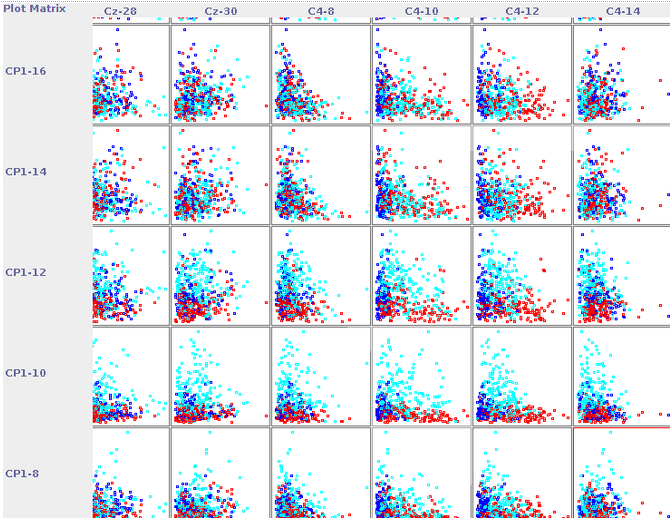
\includegraphics[width=0.31\linewidth]{img/exploratory-data-analysis/correlation1}
        \label{img:correlation1}
    }
    \subfigure[Correlation of features]
    {
        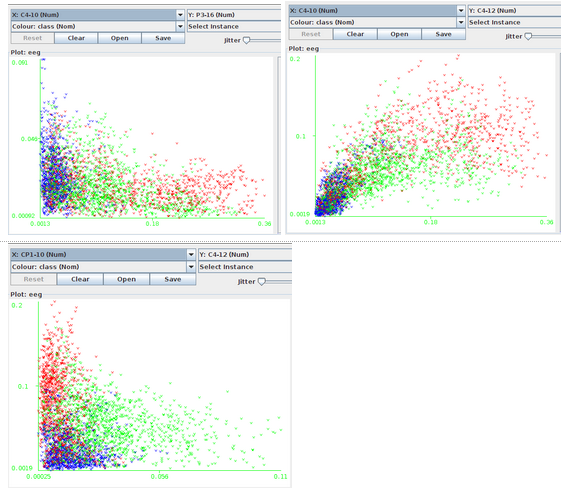
\includegraphics[width=0.31\linewidth]{img/exploratory-data-analysis/correlation2}
        \label{img:correlation2}
    }
    \subfigure[Correlation of highest ranked features using Information Gain]
    {
        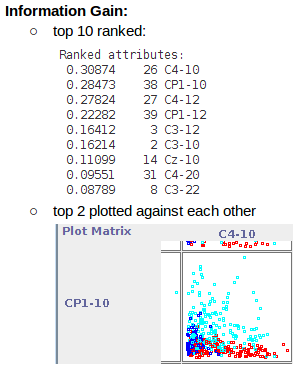
\includegraphics[width=0.31\linewidth]{img/exploratory-data-analysis/correlation3}
        \label{img:correlation3}
    }
    \caption{Correlation of Features}
    \label{img:correlation}
\end{figure}

